\documentclass[tikz, border=5pt]{standalone}
\usepackage{tikz}
\usetikzlibrary{shapes, arrows}

\begin{document}
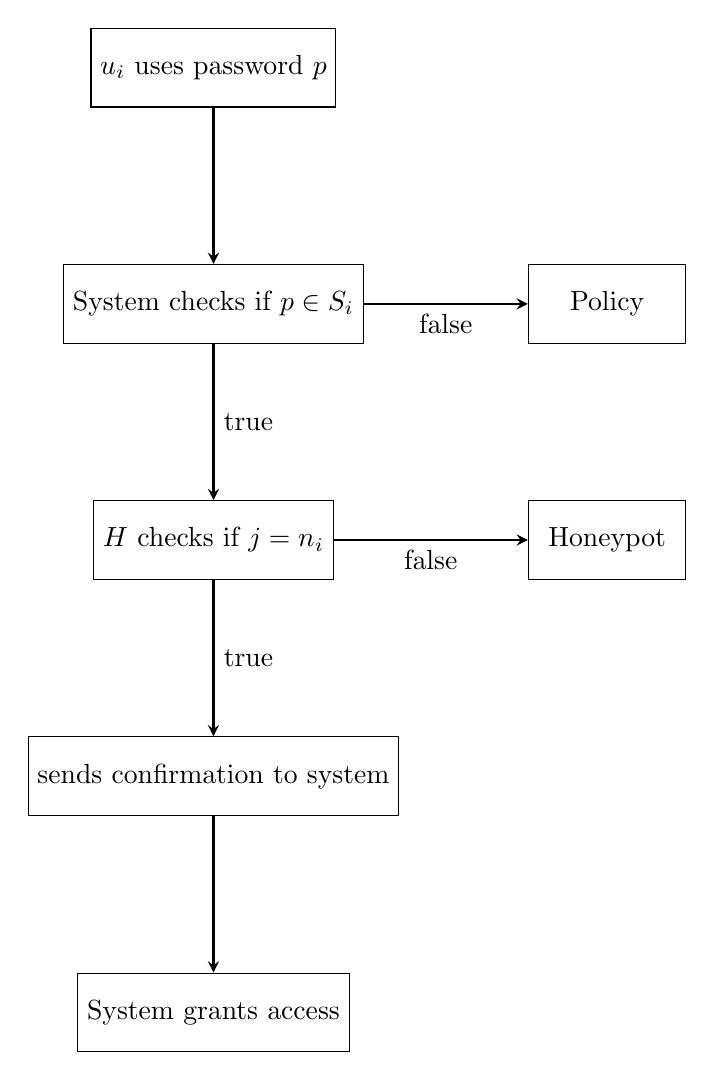
\begin{tikzpicture}[node distance=1.5cm]
    \tikzstyle{startstop} = [rectangle, draw, minimum width=2cm, minimum height=1cm, text centered, node distance=3cm]
    \tikzstyle{process} = [rectangle, draw, text centered, minimum width=2cm, minimum height=1cm, node distance=3cm]
    \tikzstyle{decision} = [rectangle, draw, text centered, minimum width=2cm, minimum height=1cm, node distance=3cm]
    \tikzstyle{arrow} = [thick,->,>=stealth]

    \node (start) [startstop] {\(u_i\) uses password \(p\)};
    \node (init) [process, below of=start] {System checks if \(p \in S_i\)};
    \node (authenticate) [process, below of=init] {\(H\) checks if \(j = n_i\)};
    \node (decision) [decision, below of=authenticate] {sends confirmation to system};
    \node (access) [process, below of=decision] {System grants access};
    \node (policy) [process, right of=init, xshift=2cm] {Policy};
    \node (honeypot) [process, right of=authenticate, xshift=2cm] {Honeypot};

    % Arrows
    \draw [arrow] (start) -- (init);
    \draw [arrow] (init) -- node[anchor=west] {true}(authenticate);
    \draw [arrow] (init) -- node[anchor=north] {false}(policy);
    \draw [arrow] (authenticate) -- node[anchor=west] {true}(decision);
    \draw [arrow] (authenticate) -- node[anchor=north] {false}(honeypot);
    \draw [arrow] (decision) -- (access);
\end{tikzpicture}
\end{document}
